\chapter{Cross-Lingual Mechanisms during GRPO Training}
\label{ch:grpo-crosslingual}

\section{Introduction}
\label{sec:grpo-intro}

\subsection{Motivation}
\label{subsec:grpo-motivation}

Chapter~\ref{ch:neurons} asked where language sits inside a fixed model and found
that editing a localized set of neurons does not change what the model does on a
task. This chapter asks a different question. Instead of probing a fixed model, we
watch how a training procedure changes a model's cross-lingual behaviour over time.
The procedure is Group Relative Policy Optimization (GRPO), a reinforcement learning
method used to fine-tune models for reasoning, and the behaviour we track is how the
model handles the same math problem posed in different languages.

There is a common claim about how multilingual models process non-English input.
The claim, which we call the Wendler three-phase hypothesis
\citep{wendler2024llamas}, is that the model maps the input into an English-aligned
space in the early layers, works in that space through the middle layers, and maps
back to the input language only in the last few layers. If this is right, then
reading out the language of the model's intermediate predictions should show English
through the body of the stack and the target language only at the end.

This matters once reinforcement learning enters. GRPO rewards the model based on
whether the final answer is correct, judged by a verifier that reads only the
answer, not the language of the reasoning. If the model could raise its reward by
leaning more on an English-aligned middle of the stack, then training might push it
in that direction and widen the gap for low-resource languages. Whether GRPO
actually changes this internal behaviour, and how its effect varies across
languages, is what we study.

\subsection{Problem Statement}
\label{subsec:grpo-problem}

We study how GRPO fine-tuning changes the cross-lingual behaviour of a multilingual
math reasoner. This breaks into the following parts.

\begin{enumerate}
	\item \textbf{Does GRPO change accuracy, and does it do so evenly across
		languages?} We track per-language accuracy across training to see how much, and
	for which languages, GRPO moves the task performance.
	
	\item \textbf{Does the model predict in English in the middle layers, and does
		GRPO change this?} The three-phase hypothesis describes an English-leaning
	middle of the stack. We check whether this is present, and whether training
	makes it stronger or weaker, using the language of the model's intermediate
	predictions.
	
	\item \textbf{Which languages does GRPO struggle with, and what is happening
		inside the model for them?} For a language that GRPO does not improve, we ask
	whether its representations are left alone or are changed without any matching
	accuracy gain, and what sets such a language apart from the rest.
\end{enumerate}

\subsection{Contributions}
\label{subsec:grpo-contributions}

This chapter reports the following.

\begin{itemize}
	\item We fine-tune Qwen2.5-7B-Instruct on the seven-language MGSM benchmark with
	GRPO and a low-rank adapter, save checkpoints across 620 gradient steps, and
	study the model along five lines: end-task accuracy, the per-layer language of
	logit-lens predictions, a three-phase categorical analysis of those predictions,
	the gap between English and the target language, and the geometry of the
	representations measured with Centred Kernel Alignment.
	
	\item We find that GRPO moves accuracy very little for any of these languages.
	Six of the seven stay in a band between about $0.72$ and $0.94$ and change by at
	most a few points over training, and Telugu stays far below the rest, at about
	$0.38$ to $0.40$, throughout.
	
	\item We find that GRPO does not cause cross-lingual collapse. The model already
	reads out as English through the early and middle layers and surfaces the target
	language only in the last few layers, and this is present from the start and
	does not change over 620 GRPO steps. Training neither builds up nor removes the
	English-leaning middle of the stack.
	
	\item We show that Telugu, the language that sits far below the rest, is also the
	one whose representations GRPO changes the most, while its accuracy does not
	move. We connect this to tokeniser coverage: Telugu has very few dedicated tokens
	in the Qwen2.5 vocabulary, and we argue that the limiting factor for GRPO here is
	the granularity of the reward signal, not language identity or a change in the
	model's internal routing.
\end{itemize}

\section{Background}
\label{sec:grpo-background}

\subsection{The Three-Phase Hypothesis}
\label{subsec:grpo-wendler}

Work on how multilingual transformers process input has suggested a three-phase
picture \citep{wendler2024llamas}. In the early layers the model maps the input
tokens into its internal representation. In the middle layers it works in a space
closer to English than to the input language, so a tool that reads out the model's
intermediate state would see English-like predictions even when the input is in
another language. In the last layers the model maps back to the input language to
produce the output. We call this the early-target, mid-English, late-target
structure.

The hypothesis matters here for two reasons. First, it makes a static prediction:
reading out the language of the model's intermediate predictions should show English
through the body of the stack and the target language only near the end. Second, and
more important for us, it raises a training question. Since the GRPO reward depends
only on the final answer and not on the language of the reasoning, training could
push the model to lean even more on an English-aligned middle. We test the static
prediction, and by tracking it across checkpoints, we test whether GRPO changes it.

\subsection{Group Relative Policy Optimization}
\label{subsec:grpo-objective}

GRPO \citep{shao2024deepseekmath} is an online policy-gradient method. For a prompt,
the policy generates a group of responses, each scored by a reward function. Instead
of using a separate value model to compute a baseline, GRPO standardizes the rewards
within the group and uses that as the advantage.

Let $\pi_\theta$ be the policy, $\pi_{\theta_{\text{old}}}$ the policy at the start
of the current rollout, and $\pi_{\text{ref}}$ a frozen reference policy. For a
prompt $i$, the policy generates $G$ responses $\{y_{i,j}\}_{j=1}^G$, and each
receives a scalar reward $R_i^j$. The group-relative advantage standardizes the
rewards within the group:
\begin{equation}
	\mu^i = \frac{1}{G} \sum_{j=1}^{G} R_i^j, \qquad
	\sigma^i = \sqrt{\frac{1}{G} \sum_{j=1}^{G} (R_i^j - \mu^i)^2}, \qquad
	A_i^j = \frac{R_i^j - \mu^i}{\sigma^i}.
	\label{eq:grpo-advantage}
\end{equation}
The advantage is the same for every token in a response. The per-response objective
uses a clipped policy ratio with a KL penalty against the reference policy, in the
usual GRPO form, and the per-batch loss averages this over the group and the batch:
\begin{equation}
	\mathcal{L}_{\text{GRPO}}(\theta) = -\frac{1}{B} \sum_{i=1}^{B} \frac{1}{G} \sum_{j=1}^{G} \mathcal{L}_{i,j}^{\text{resp}},
	\label{eq:grpo-loss}
\end{equation}
where $B$ is the batch size. We use a clipping range $\epsilon = 0.2$ and a KL
coefficient $\beta = 0.04$. The reward is binary, based on whether an external judge
accepts the final answer, and is described in Section~\ref{subsec:grpo-reward}.

\subsection{Tools for Looking Inside the Model}
\label{subsec:grpo-tools}

Two tools from Chapter~\ref{ch:related-work} are used throughout. The logit lens
\citep{nostalgebraist2020logitlens} reads out what the model would predict at an
intermediate layer by applying the model's final normalization and output head to
that layer's residual-stream activation, giving a distribution over the vocabulary
at each layer. We use it to ask, at each layer, which language the model's predicted
token belongs to. Centred Kernel Alignment (CKA)
\citep{kornblith2019similarity} measures how similar two sets of representations are,
in a way that does not change under rotation or uniform scaling. We use it to compare
a language's representations with English at each layer, and to compare a language's
representations at a training checkpoint with the same language in the base model,
which measures how far training has moved them.

\section{Experimental Setup}
\label{sec:grpo-setup}

\subsection{Dataset and Prompt Format}
\label{subsec:grpo-data}

We use the Multilingual Grade School Math (MGSM) benchmark \citep{shi2022mgsm},
which translates grade-school math word problems into several languages. We use
seven: English (en), Bengali (bn), Telugu (te), Thai (th), Russian (ru), Japanese
(ja), and Chinese (zh). These cover a range of scripts and a range of resource
levels with respect to the Qwen2.5 tokeniser. For each language we use 200 examples
for training and 50 for evaluation, giving $1{,}400$ training and $350$ evaluation
examples. A small held-out pool of eight examples per language with hand-written
chain-of-thought solutions is kept aside for use as few-shot demonstrations.

Each prompt uses a one-shot format: an instruction in English describing the output
format, one worked example in the target language from the held-out pool, then the
question, ending with the marker \texttt{Step-by-step Answer:}. The instruction line
and the field headers (\texttt{Question:}, \texttt{Step-by-step Answer:},
\texttt{Final Answer:}) are kept in English for every language; only the question
text and the worked example are in the target language. The final answer must be
written as an English integer on a line \texttt{Final Answer: <number>}. This gives
a clear target for the answer extractor and roughly matches how multilingual
reasoners are used in practice, where some English context is usually present.

\subsection{Tokeniser Coverage}
\label{subsec:grpo-coverage}

The Qwen2.5 tokeniser does not give the same number of dedicated tokens to every
script. Counting the vocabulary tokens whose decoded bytes contain at least one
character in a language's script gives the approximate coverage in
Table~\ref{tab:grpo-coverage}. The gap is large: Thai has on the order of $2{,}500$
tokens, Bengali about $46$, and Telugu about $14$. As the results will show, this
gap lines up with the one language GRPO cannot lift.

% TABLE 4.1 (tokeniser coverage). Booktabs. Label: tab:grpo-coverage
\begin{table}[t]
	\centering
	\renewcommand{\arraystretch}{1.2}
	\begin{tabular}{llc}
		\toprule
		\textbf{Language} & \textbf{Coverage class} & \textbf{Script tokens (approx.)} \\
		\midrule
		Chinese  & High (multi-byte CJK base) & $\sim 25{,}000$ \\
		Japanese & High (kanji, kana)         & $\sim 6{,}000$  \\
		Russian  & High (Cyrillic block)      & $\sim 4{,}000$  \\
		Thai     & Mid                        & $\sim 2{,}500$  \\
		Bengali  & Low                        & $\sim 46$       \\
		Telugu   & Very low                   & $\sim 14$       \\
		English  & Bulk of the vocabulary     & ---             \\
		\bottomrule
	\end{tabular}
	\caption{Approximate number of Qwen2.5 vocabulary tokens whose script range
		overlaps each studied language. The order-of-magnitude gap between Thai and the
		two Indic scripts (Bengali, Telugu) lines up with the per-language outcome.}
	\label{tab:grpo-coverage}
\end{table}

\subsection{Model}
\label{subsec:grpo-model}

The policy model is Qwen2.5-7B-Instruct, a decoder-only transformer with $L=28$
layers and residual-stream width $d=3584$. The reference model for the KL term is a
frozen copy of the same model. To fit the compute budget, we attach a low-rank
adapter \citep{hu2022lora} of rank $r=64$ with scaling factor $\alpha=16$ and dropout
$0.05$ to the attention projections (\texttt{q\_proj}, \texttt{k\_proj},
\texttt{v\_proj}, \texttt{o\_proj}) of every layer. Only the adapter is updated; the
base weights stay frozen. The reference model is the same base model with the adapter
disabled, which is the unmodified Qwen2.5.

\subsection{Reward, Generation, and Training}
\label{subsec:grpo-reward}

The training reward comes from a verifier that reads the model's chain-of-thought and
checks whether it reaches the correct final answer. The verifier combines a regex
match for the answer line with a judge model (GPT-4o-mini) for the cases where the
formatting differs but the answer may still be correct. The reward is binary: $1$ if
the answer is accepted, $0$ otherwise or if the response cannot be parsed. We use a
judge in addition to a string match because early in training the model often
produces answers with small formatting differences, such as a stray period or a digit
in a foreign script, that a string match alone would wrongly reject.

During rollouts and evaluation, responses are generated with temperature $0.7$,
nucleus sampling with $p=0.95$, and up to $512$ new tokens, with generation stopped
shortly after the first \texttt{Final Answer:} marker. The group size is $G=4$, so
the policy generates four responses per prompt, and the group-relative advantage of
Equation~\ref{eq:grpo-advantage} is computed over these four. The remaining settings
are in Table~\ref{tab:grpo-hyperparams}.

% TABLE 4.2 (training hyperparameters). Booktabs. Label: tab:grpo-hyperparams
\begin{table}[t]
	\centering
	\renewcommand{\arraystretch}{1.2}
	\begin{tabular}{ll}
		\toprule
		\textbf{Setting} & \textbf{Value} \\
		\midrule
		Policy model        & Qwen2.5-7B-Instruct ($L=28$, $d=3584$) \\
		Reference model     & frozen Qwen2.5-7B-Instruct (adapter disabled) \\
		Verifier            & regex match + GPT-4o-mini judge \\
		LoRA rank $r$       & 64 \\
		LoRA scaling $\alpha$ & 16 \\
		LoRA dropout        & 0.05 \\
		LoRA target modules & \texttt{q\_proj}, \texttt{k\_proj}, \texttt{v\_proj}, \texttt{o\_proj} \\
		Group size $G$      & 4 \\
		Clipping range $\epsilon$ & 0.2 \\
		KL coefficient $\beta$    & 0.04 \\
		Optimizer           & AdamW \\
		Peak learning rate  & $1\times10^{-5}$ \\
		Gradient clipping   & norm $1.0$ \\
		Batch size $B$      & 8 prompts ($\times\,G=4$ rollouts) \\
		Total steps         & 620 \\
		Temperature         & 0.7 \\
		Nucleus sampling $p$ & 0.95 \\
		Max new tokens      & 512 \\
		\bottomrule
	\end{tabular}
	\caption{GRPO training and generation settings.}
	\label{tab:grpo-hyperparams}
\end{table}

We optimize with AdamW at a peak learning rate of $1\times10^{-5}$ and gradient
clipping at norm $1.0$, for $620$ gradient steps, with $B=8$ prompts and $G=4$
rollouts each per step. We save a checkpoint every $20$ steps, where step $0$ is the
base model with the adapter zero-initialized, so it produces the same outputs as the
unmodified Qwen2.5. The analysis runs on the resulting $30$ checkpoints from step $0$
to step $620$.

\subsection{Analysis Pipeline}
\label{subsec:grpo-pipeline}

At each checkpoint we evaluate on the 350-prompt evaluation set, generating with
greedy decoding so the evaluation chain-of-thought is deterministic. For each prompt
we record the prompt language, the generated chain-of-thought, and the
residual-stream activations at every layer, so the measurements can be computed from
the cached file without running the model again. The per-layer quantities come from
the logit lens: for every layer $i$ and every chain-of-thought position $k$, we take
the activation, pass it through the model's final normalization and output head, and
form a distribution over the full vocabulary. This is the basis for the
language-identity and gap measurements below.

\section{The Five Measurements}
\label{sec:grpo-axes}

We look at the checkpoint sequence in five ways.

\paragraph{(i) End-task accuracy.}
For each checkpoint and language, the fraction of evaluation problems the model
solves, as judged by the verifier. This tells us whether GRPO improves a language.

\paragraph{(ii) Per-layer language distribution.}
Using the logit-lens distribution, at each layer and checkpoint we measure how much
of the model's prediction mass falls on each language, averaged over chain-of-thought
positions and prompts, renormalized over the seven studied languages. Reading this by
layer shows which language the model predicts in at each depth; reading it across
checkpoints shows whether GRPO changes that.

\paragraph{(iii) Three-phase analysis.}
We split the stack into early, middle, and late phases, and for each phase measure
how often the model's top-1 logit-lens prediction is a token of a given language. We
also report this at the last few layers on their own. This is a coarser version of
(ii) that maps onto the early-target, mid-English, late-target structure.

\paragraph{(iv) English-minus-target gap.}
For each layer and checkpoint we compute the gap between the fraction of top-1
predictions that are English and the fraction that are the target language, averaged
over positions and prompts. A positive gap means English leads the target language at
that depth. This summarizes the English lead in one number per layer.

\paragraph{(v) Representation geometry.}
Using CKA on the mean chain-of-thought activations, we measure two things. The
cross-lingual similarity compares each language with English at each layer and
checkpoint. The within-language drift compares each language at a checkpoint with the
same language at step $0$, which measures how far training has moved it. Together
these show whether a language that does not improve is left alone or changed without
benefit.

\section{Results}
\label{sec:grpo-results}

\subsection{Accuracy over Training}
\label{subsec:grpo-acc}

Figure~\ref{fig:grpo-accuracy} shows per-language accuracy across the 620 GRPO steps,
and Table~\ref{tab:grpo-acc} gives the first and last checkpoint values. The main
point is that GRPO moves accuracy very little. Six of the seven languages sit in a
band between about $0.72$ and $0.94$ and wiggle by a couple of points across training
without any clear upward trend; their first-to-last changes are between $0$ and
$0.04$. Telugu sits well below the rest, at about $0.38$ to $0.40$, and stays there for the
whole run. So on this task GRPO does not lift the languages much, and Telugu in
particular stays far below the others throughout.

% FIGURE 4.1 -- include here.
% PLOT: plots/plot_accuracy_gpt/plot_accuracy_gpt.png
% Suggested filename: fig_grpo_accuracy.png
\begin{figure}[t]
	\centering
	 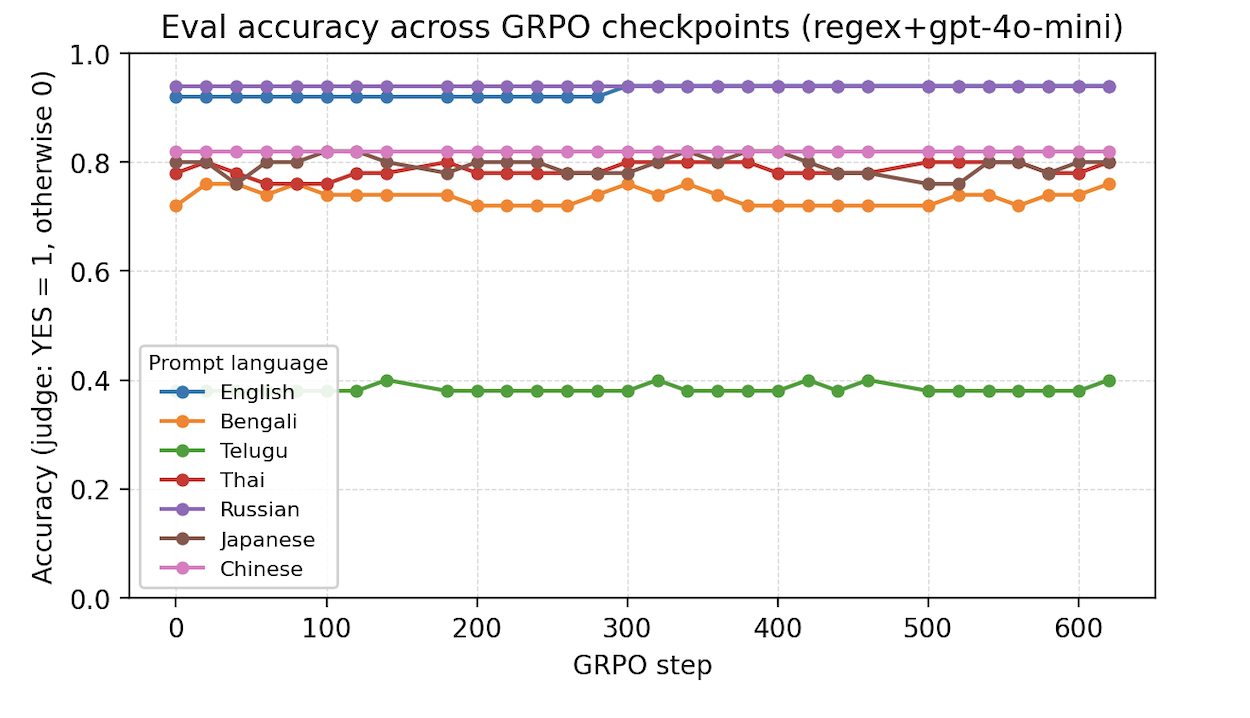
\includegraphics[width=0.8\linewidth]{Chapters/Chapter_4/accuracy_gpt.png}
	\caption{Per-language evaluation accuracy across GRPO training steps, scored by
		the regex-plus-judge verifier. Six languages stay in a band between about $0.72$ and $0.94$ with
		little change over training; Telugu stays at about $0.38$ to $0.40$ throughout.}
	\label{fig:grpo-accuracy}
\end{figure}

% TABLE 4.3 (accuracy first vs last). Booktabs. Label: tab:grpo-acc
\begin{table}[t]
	\centering
	\renewcommand{\arraystretch}{1.2}
	\begin{tabular}{lccc}
		\toprule
		\textbf{Language} & \textbf{Step 0} & \textbf{Step 620} & \textbf{Change} \\
		\midrule
		English  & 0.92 & 0.94 & $+0.02$ \\
		Russian  & 0.94 & 0.94 & $+0.00$ \\
		Chinese  & 0.82 & 0.82 & $+0.00$ \\
		Japanese & 0.80 & 0.80 & $+0.00$ \\
		Thai     & 0.78 & 0.80 & $+0.02$ \\
		Bengali  & 0.72 & 0.76 & $+0.04$ \\
		Telugu   & 0.38 & 0.40 & $+0.02$ \\
		\bottomrule
	\end{tabular}
	\caption{Evaluation accuracy at the first and last checkpoint. The changes are
		small for every language, and Telugu stays far below the rest.}
	\label{tab:grpo-acc}
\end{table}

\subsection{Which Language Does the Model Predict in at Each Layer?}
\label{subsec:grpo-logitlens}

Figure~\ref{fig:grpo-logitlens} shows, by layer and by training step, how much of the
model's logit-lens prediction mass falls on each language, renormalized over the
seven studied languages, for a Telugu prompt and a Thai prompt. The pattern is the
same across prompt languages. For a non-English prompt, the early and middle layers
put most of their renormalized mass on English, with the prompt's own language near
zero, and the target language appears only in the last two or three layers, where
English is still comparable to it. So the model reads out as English through the body
of the stack and surfaces the target language only at the very end.

For this chapter the important thing is how this changes with training, which is to
say it does not. Across all $620$ GRPO steps the per-layer pattern is flat: the
English mass in the early and middle layers does not grow, and the point at which the
target language appears does not move. GRPO does not build up the English-leaning
middle of the stack, and it does not remove it. This holds for every language.

% FIGURE 4.2 -- include here.
% PLOT: from plots/plot1/. Recommended: a small grid of layer-vs-checkpoint heatmaps
% for the low-resource case, e.g. plot1_heatmap_prompt-te_target-en.png and
% plot1_heatmap_prompt-te_target-te.png, to show English high through the body and
% Telugu near zero until the top. Optionally add a high-resource case for contrast.
% Suggested filename: fig_grpo_logitlens.png
\begin{figure}[ht]
	\centering
	 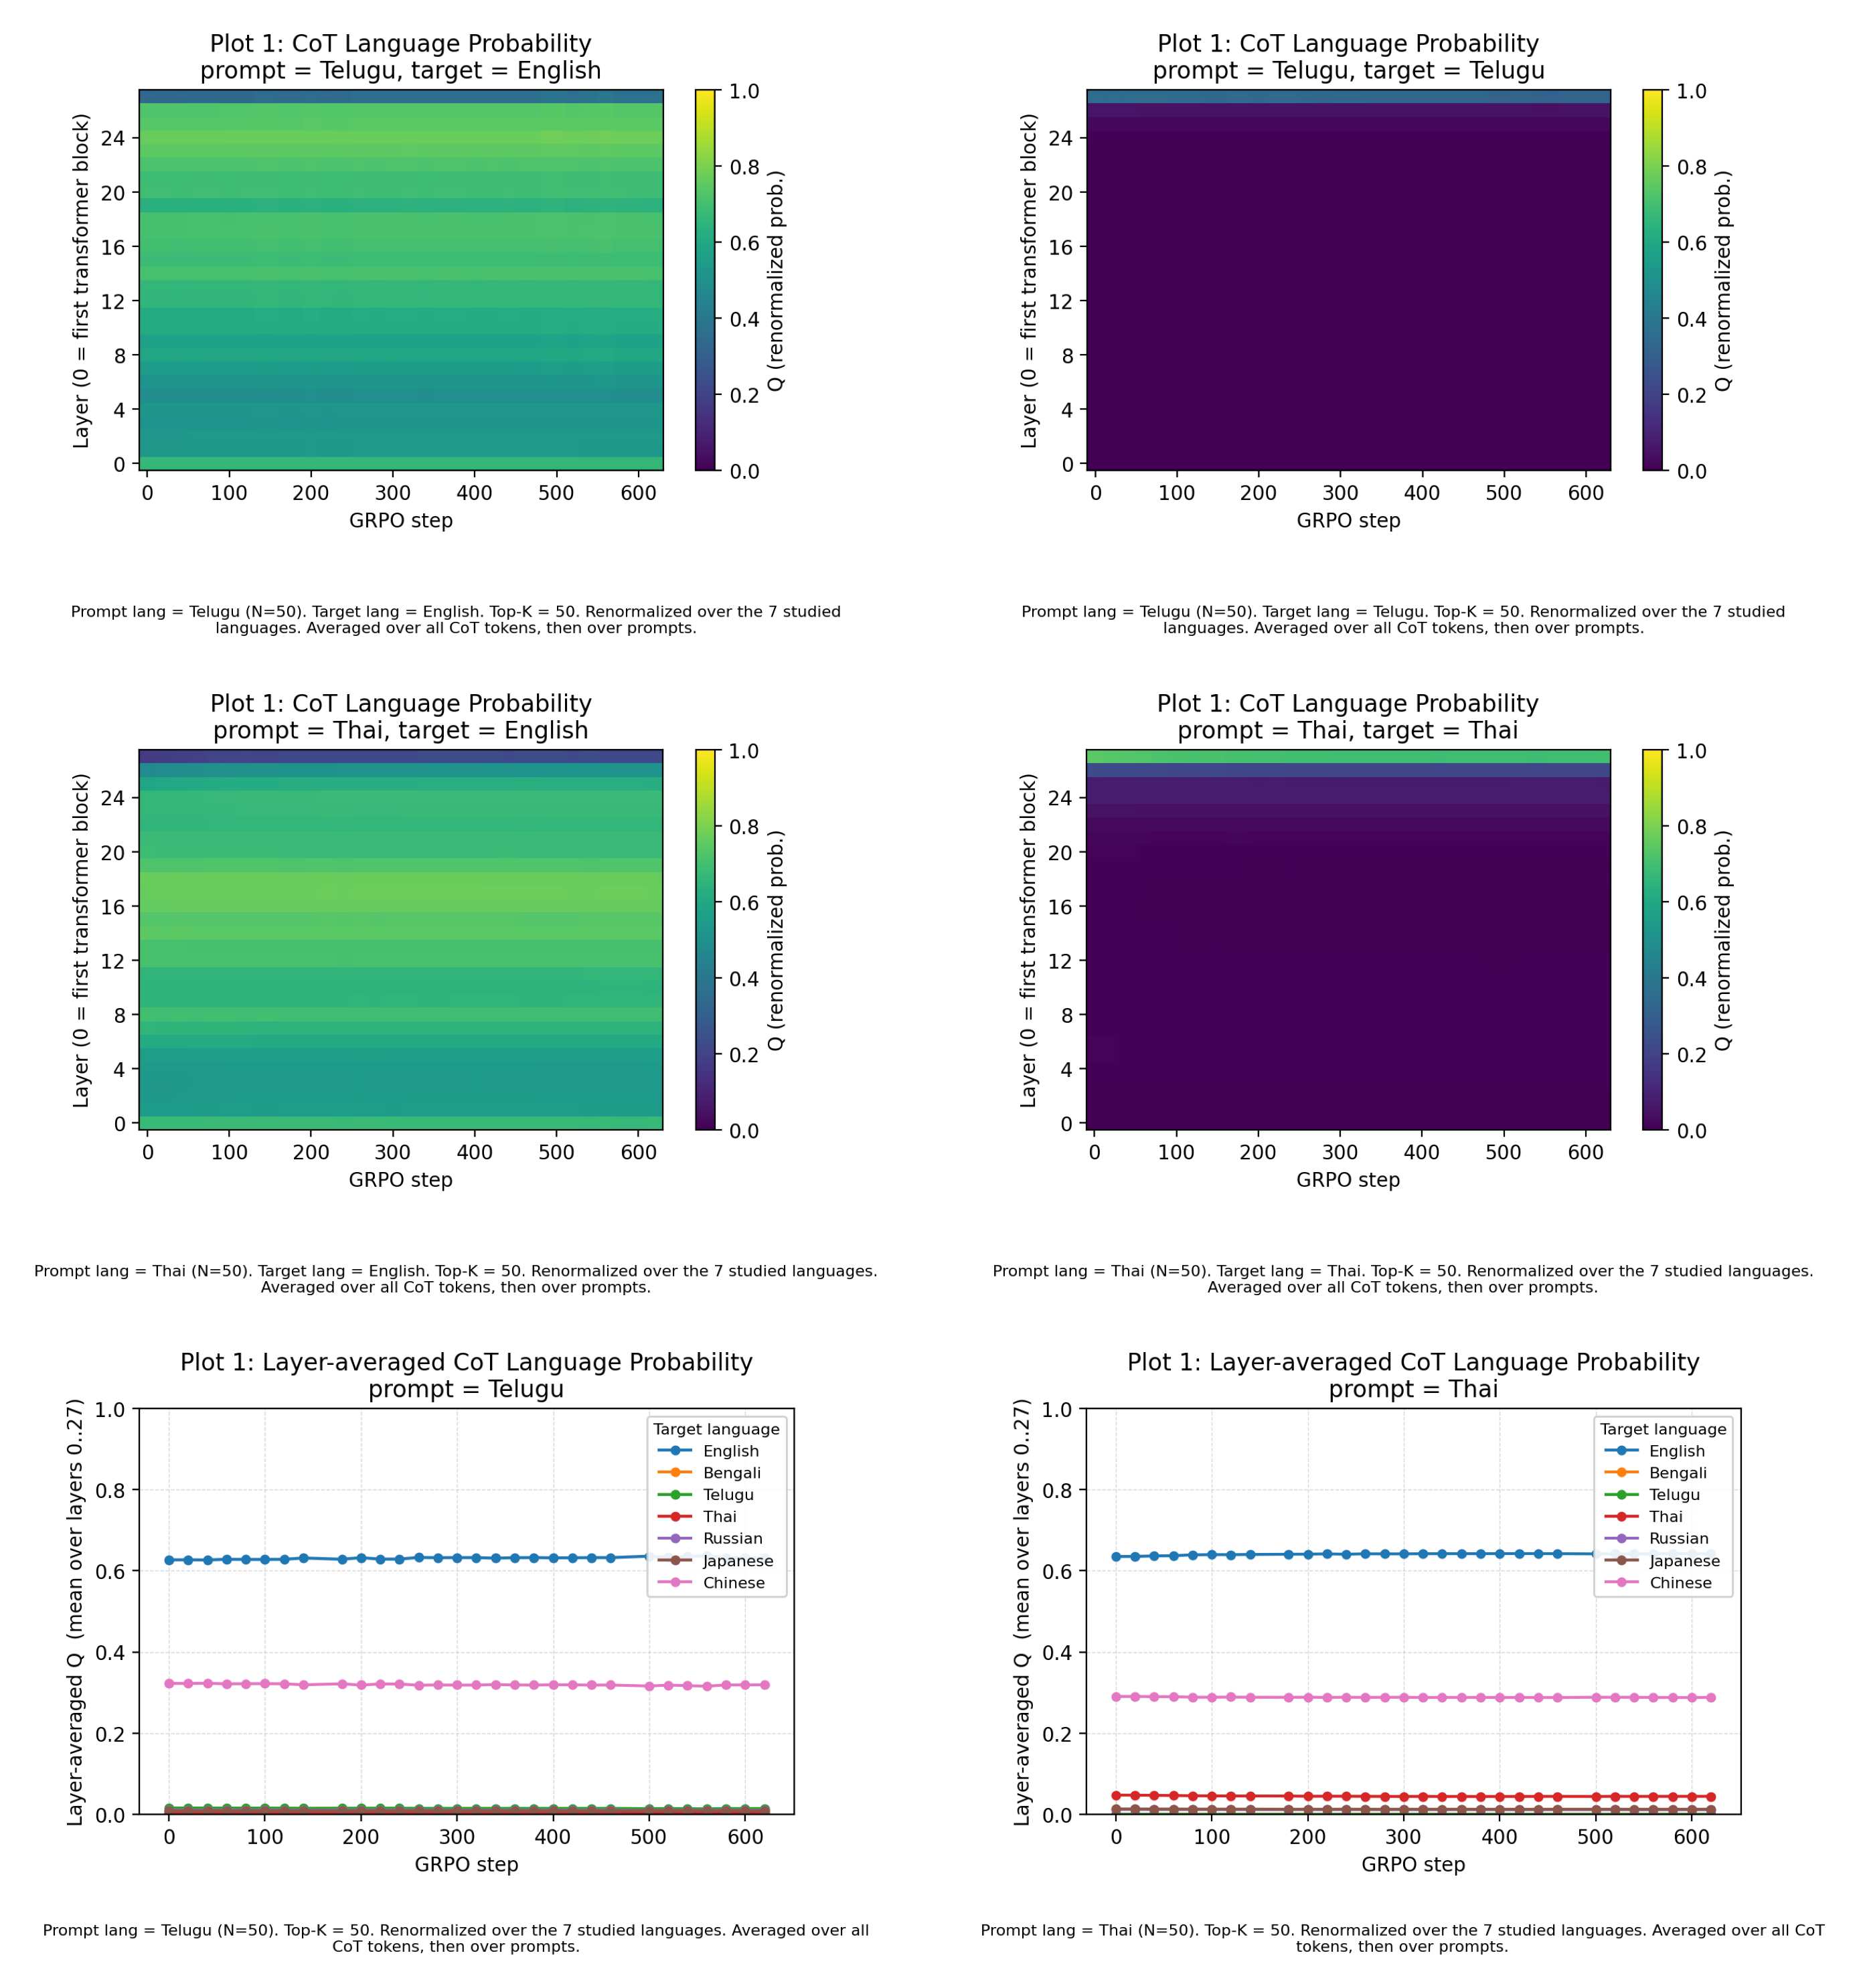
\includegraphics[width=0.8\linewidth]{Chapters/Chapter_4/Figures/combined_plot1.png}
	\caption{Logit-lens language probability for a Telugu prompt (left column) and a
		Thai prompt (right column). The top row is the renormalized probability of an
		English readout, by layer (vertical) and GRPO step (horizontal). The middle row is
		the same for the prompt's own-language readout. The bottom row averages the
		probability over layers and plots it against GRPO step, with one curve per target
		language. For both prompts, English probability is high through the early and middle
		layers while the prompt's own language stays near zero until the last two or three
		layers. All panels are flat across training, so GRPO does not change this pattern.}
	\label{fig:grpo-logitlens}
\end{figure}

\subsection{Three-Phase Analysis and the English Lead}
\label{subsec:grpo-threephase}

Figure~\ref{fig:grpo-threephase} gives the coarser categorical view, the fraction of
layers in each phase whose top-1 logit-lens prediction is a token of a given language,
together with the same at the last few layers. It confirms the picture above. English
is the most common top-1 prediction in the early and middle phases, with its share
highest in the middle phase. The target language appears mainly in the late phase, and
the two prompts differ at the very end: for Thai the target rises clearly at the last
layer and overtakes English, while for Telugu it stays low throughout.

Figure~\ref{fig:grpo-gap} states the same thing as one number per layer: the gap
between the English fraction and the target fraction of top-1 predictions. The gap is
positive through the early and middle layers for both prompts, meaning English leads
there. It is largest in the middle layers, around $0.55$ to $0.62$, and smaller in the
early and late layers. At the very end the two prompts differ: for Telugu the gap stays
positive, so English keeps the lead, while for Thai the gap turns negative at the last
layer, where Thai overtakes English. As with the other measurements, the gap is flat
across the $620$ steps, so GRPO does not change it.

% FIGURE 4.3 -- include here.
% PLOT: from plots/plot2/. Use plot2_lineplot_prompt-te.png (low-resource case),
% optionally beside plot2_lineplot_prompt-th.png.
% Suggested filename: fig_grpo_threephase.png
\begin{figure}[ht]
	\centering
	 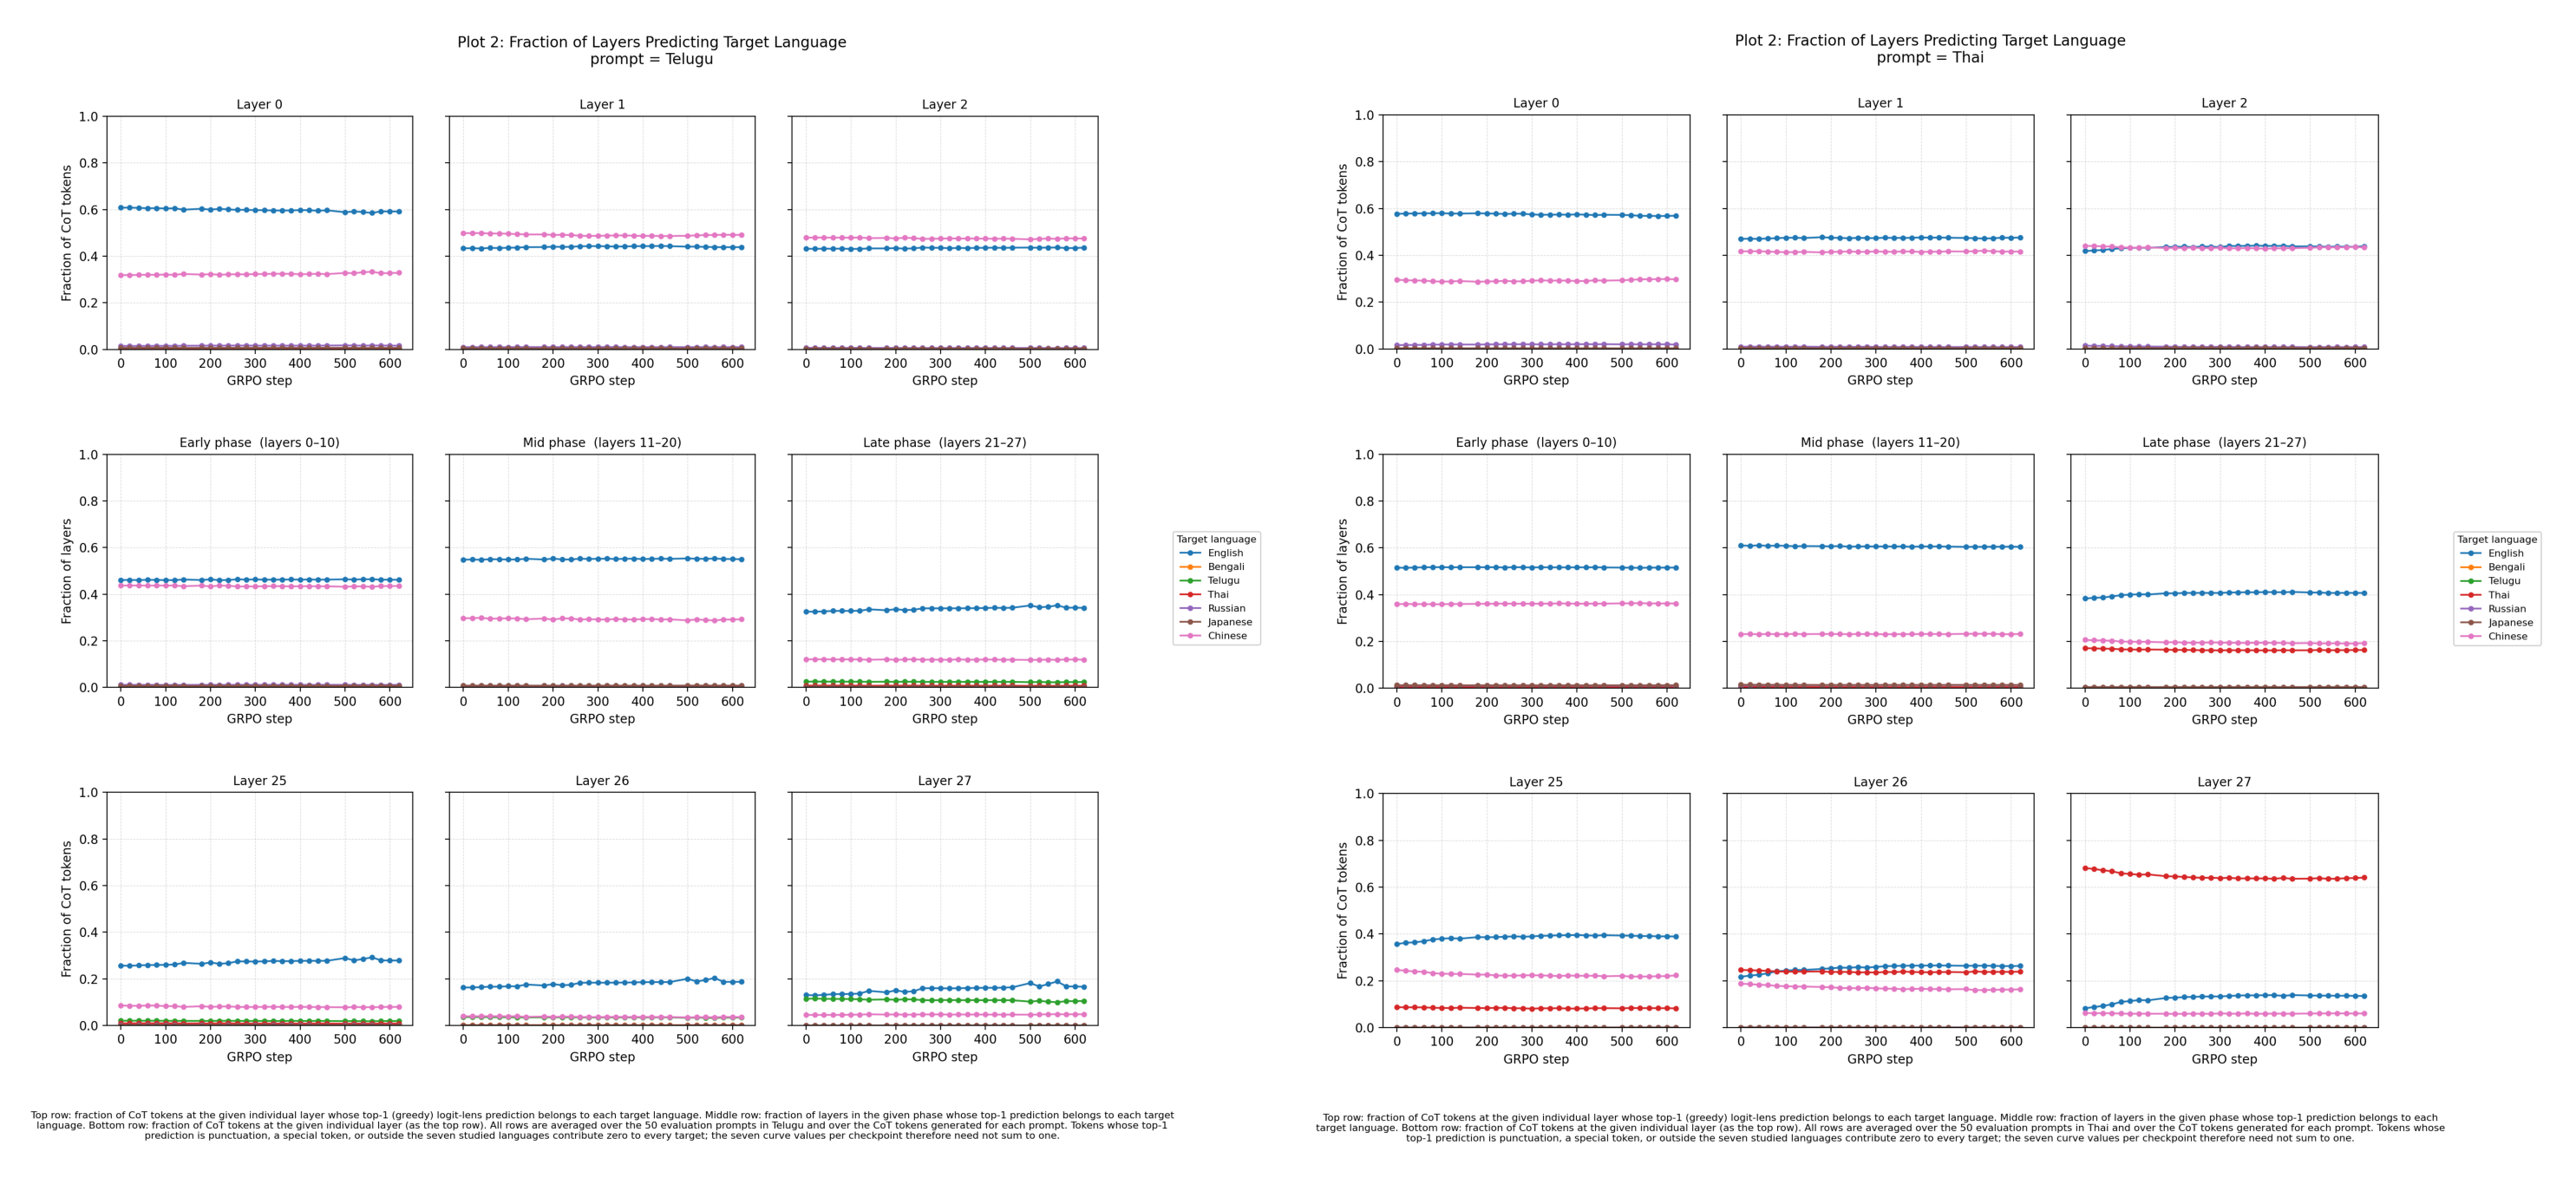
\includegraphics[width=\linewidth]{Chapters/Chapter_4/Figures/combined_plot2.png}
	\caption{Fraction of top-1 logit-lens predictions belonging to each target
		language, across GRPO steps, for a Telugu prompt (left block) and a Thai prompt
		(right block). Within each block, the top row is the first few individual layers,
		the middle row is the early, middle, and late phases, and the bottom row is the
		last few individual layers. English leads the early and middle phases for both
		prompts. The target language appears only in the late phase and final layers: for
		Thai it rises clearly at the last layer, while for Telugu it stays low throughout.
		The curves do not change over training.}
	\label{fig:grpo-threephase}
\end{figure}

% FIGURE 4.4 -- include here.
% PLOT: from plots/plot2_gap/. Use plot2_gap_lineplot_prompt-te.png, optionally beside
% another language. (This is the English-minus-target gap per phase / per layer.)
% Suggested filename: fig_grpo_gap.png
\begin{figure}[ht]
	\centering
	 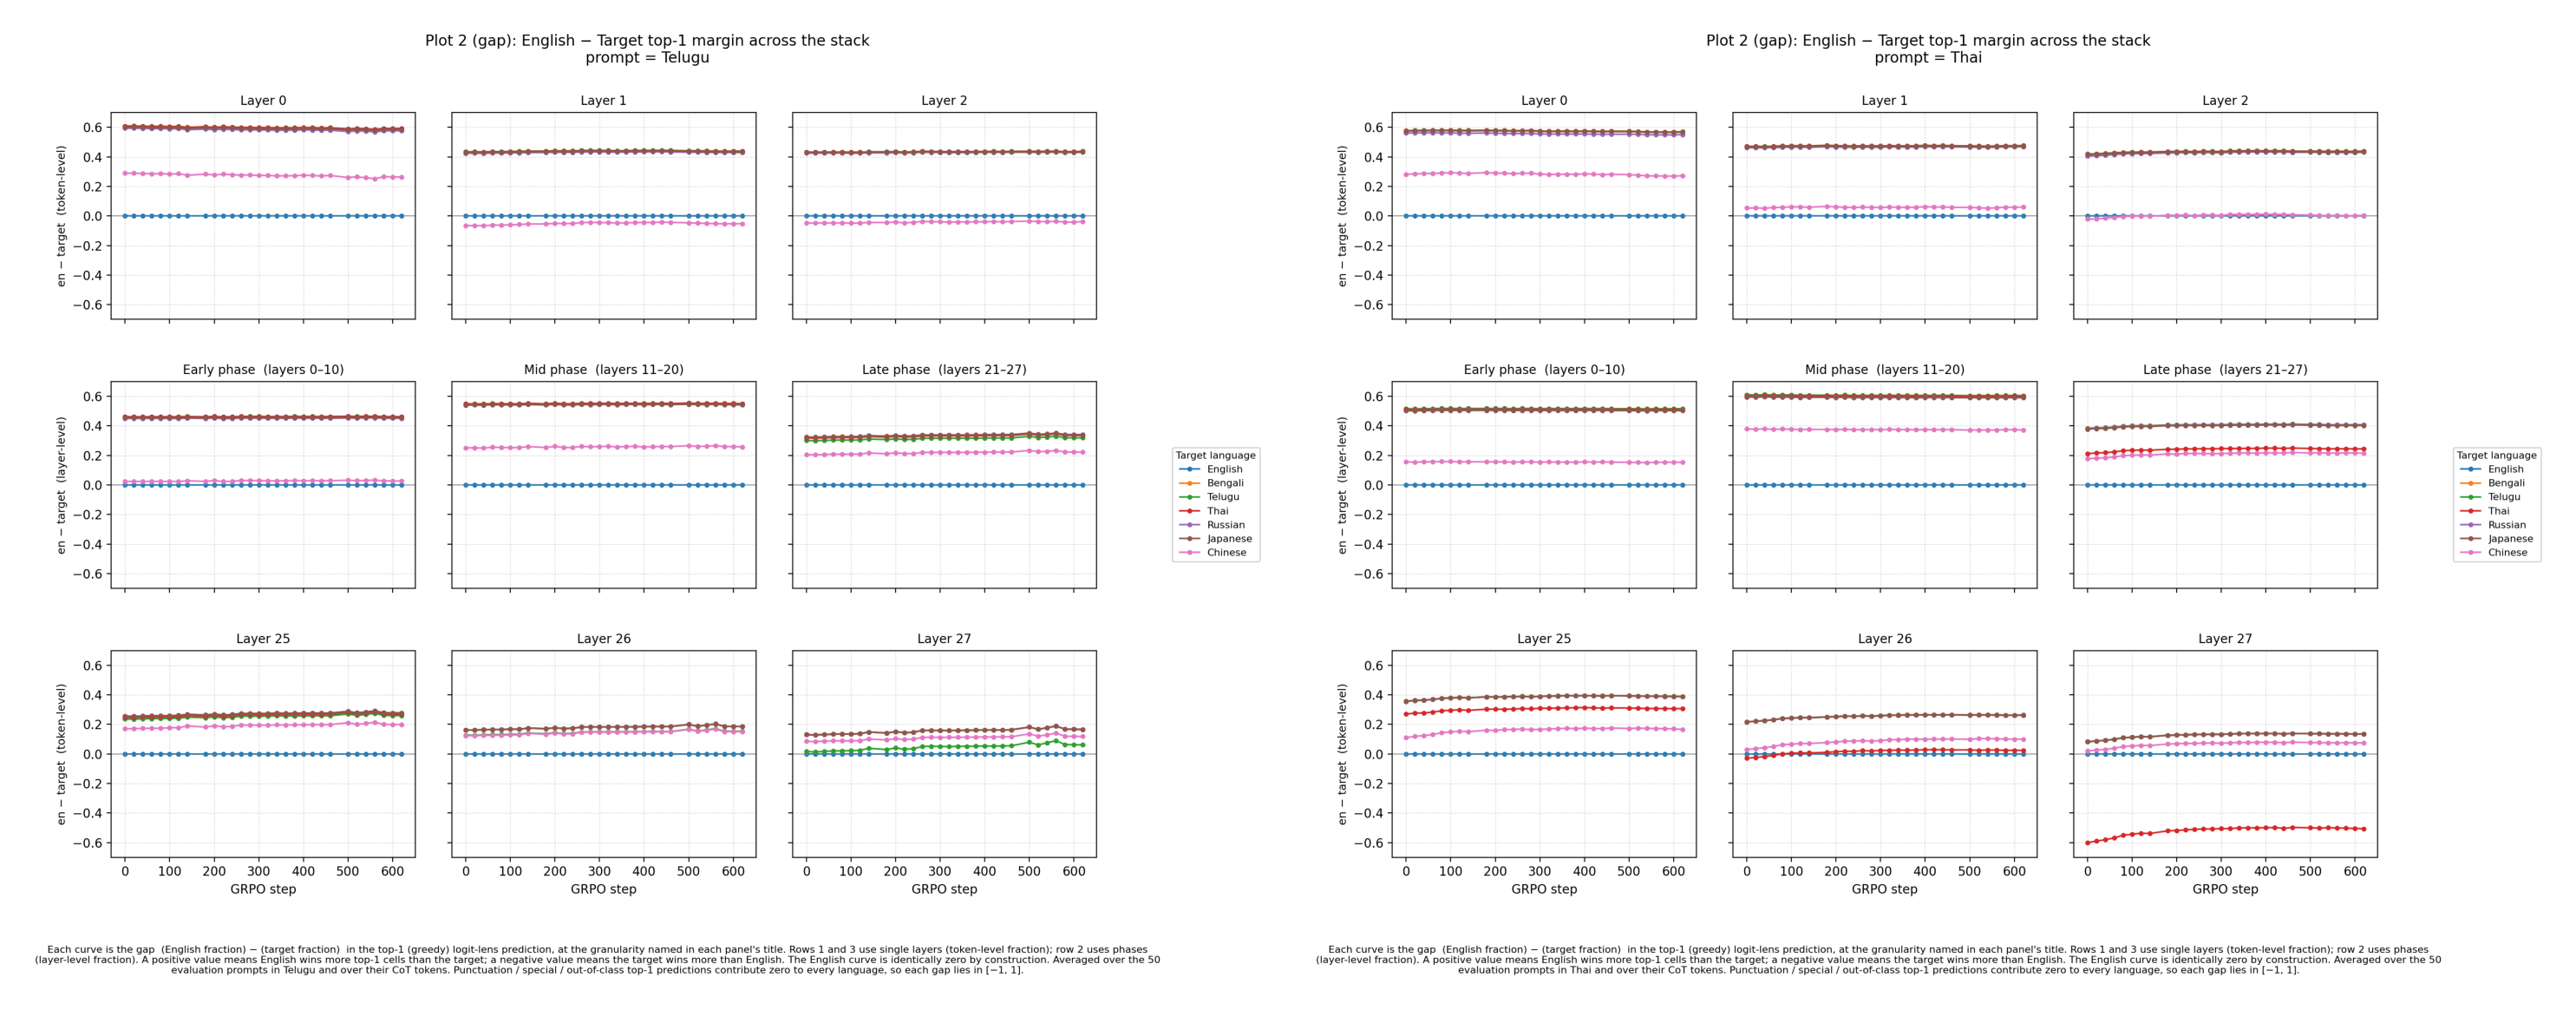
\includegraphics[width=\linewidth]{Chapters/Chapter_4/Figures/combined_plot2_gap.png}
	\caption{Gap between the English fraction and the target fraction of top-1
		logit-lens predictions, across GRPO steps, for a Telugu prompt (left block) and a
		Thai prompt (right block). A positive gap means English wins more top-1 predictions
		than the target language; a negative gap means the target wins. Within each block,
		the top row is the first few individual layers, the middle row is the early,
		middle, and late phases, and the bottom row is the last few individual layers. The
		gap is positive through the early and middle layers for both prompts, so English
		leads there. At the final layers the two prompts differ: for Thai the gap turns
		negative at the last layer, where Thai overtakes English, while for Telugu it stays
		positive throughout. The curves do not change over training.}
	\label{fig:grpo-gap}
\end{figure}

\subsection{Representation Geometry}
\label{subsec:grpo-geometry}

The measurements so far show that GRPO does not change the model's per-layer language
behaviour. The last one shows where its effect does appear, and it singles out
Telugu. Figure~\ref{fig:grpo-cka} shows two CKA measurements.

The cross-lingual similarity (left) compares each language's representations with
English, layer-averaged, across training. The curves are flat over the $620$ steps,
so training does not pull the languages closer to or further from English in
representation space. They differ by language in a way that tracks coverage: the two
low-coverage Indic languages, Telugu and Bengali, are least similar to English (around
$0.10$ and $0.15$), Russian is in the middle (around $0.32$), and Thai, Japanese, and
Chinese are highest (around $0.40$).

The within-language drift (right) compares each language at a checkpoint with the same
language at step $0$, so a lower value means training has moved it more. Telugu stands
out. Every other language stays above about $0.90$ for the whole run, meaning their
representations barely move. Telugu drops well below the rest, reaching about $0.63$ at
its lowest before settling near $0.78$. So the one language that sits far below the
others in accuracy, and does not improve, is also the one whose representations GRPO
disturbs the most. The training signal is clearly reaching Telugu and changing its
representations; it is just not turning into any accuracy gain.

% FIGURE 4.5 -- include here.
% PLOT: plots/plot4/plot4_lineplot.png (cross-lingual CKA vs English) and
% plots/plot4/plot4_drift_lineplot.png (within-language drift vs step 0), side by side.
% Suggested filename: fig_grpo_cka.png
\begin{figure}[ht]
	\centering
	 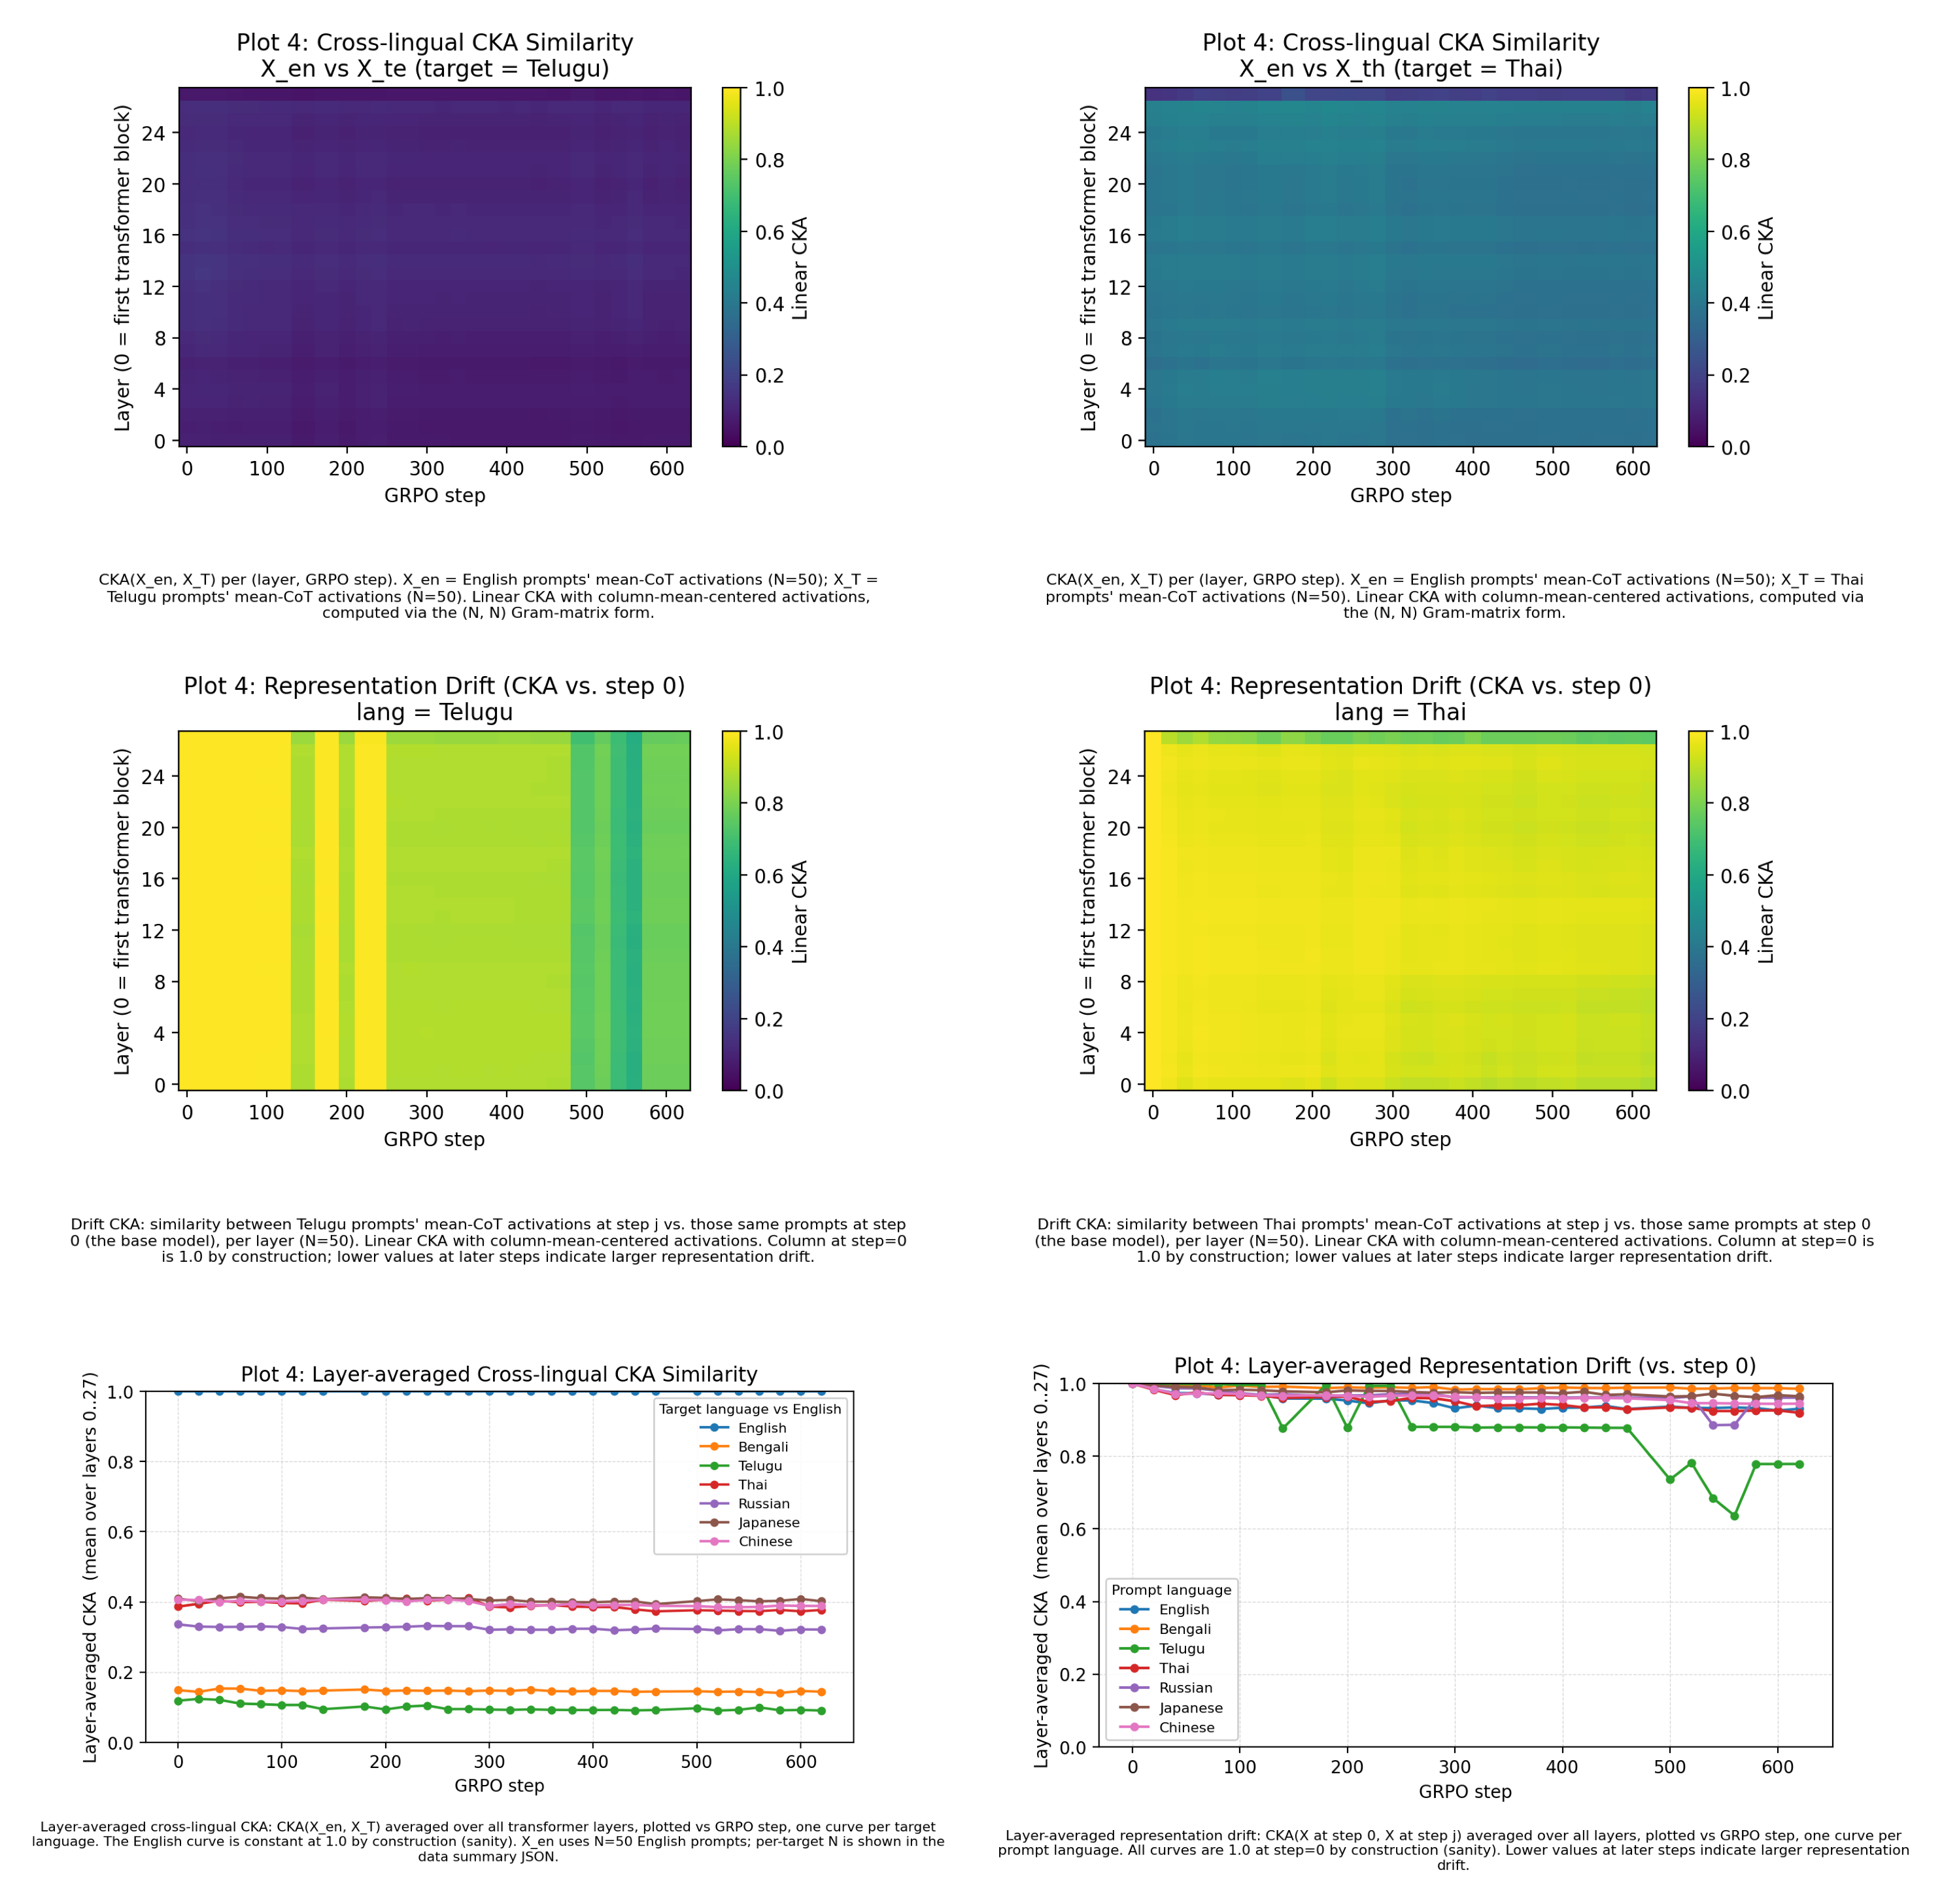
\includegraphics[width=0.8\linewidth]{Chapters/Chapter_4/Figures/combined_plot4.png}
	\caption{Representation similarity measured with CKA, across GRPO steps. The top
		row is the cross-lingual similarity between each prompt language and English, by
		layer (vertical) and GRPO step (horizontal), for Telugu (left) and Thai (right);
		Thai is more similar to English than Telugu at every layer. The middle row is the
		within-language drift, the similarity between a language's representations at a
		given step and at step $0$, for Telugu (left) and Thai (right); a lower value means
		training has moved the representations more. The bottom row gives the
		layer-averaged versions across all languages: cross-lingual similarity to English
		(left) and within-language drift (right). The low-coverage Indic languages, Telugu
		and Bengali, are least similar to English, and Telugu drifts the most over
		training, while every other language barely moves. All curves are flat in the
		cross-lingual similarity, so training does not change how close the languages sit
		to English.}
	\label{fig:grpo-cka}
\end{figure}

\section{Discussion}
\label{sec:grpo-discussion}

\subsection{GRPO Does Not Cause Cross-Lingual Collapse}
\label{subsec:grpo-no-collapse}

We set out to test whether GRPO, by rewarding only the final answer, pushes the model
toward an English-aligned middle of the stack and widens the gap for low-resource
languages over training. The results do not support this. The model does read out as
English through the early and middle layers and surfaces the target language only at
the end, which matches the static three-phase picture, but this is already present in
the base model at step $0$ and does not change over $620$ GRPO steps. The per-layer
distribution, the three-phase commitment, and the English-minus-target gap are all
flat in training. GRPO does not build up the English-leaning middle, and it does not
collapse the low-resource languages into it. Whatever that part of the stack is doing,
GRPO leaves it as it was.

\subsection{Tokeniser Coverage and the Telugu Case}
\label{subsec:grpo-coverage-discussion}

If GRPO is not changing the internal routing, what sets Telugu apart? Telugu sits far
below every other language in accuracy and does not improve, and it is also the one
whose representations GRPO moves the most. The geometry points to coverage: Telugu and
Bengali, the two languages with the fewest dedicated tokens, are the least similar to
English in representation space, and Telugu, with only about $14$ tokens, is the one
that drifts most while gaining nothing.

The reading we draw is that the limiting factor for GRPO here is the granularity of
the reward signal it can act on. When a language has very few dedicated tokens, its
text is broken into long, coarse byte sequences, and the reward, which depends on
producing a correct final answer, cannot be turned into a useful per-token gradient.
Training still moves the representations, as the Telugu drift shows, but the movement
does not line up with task competence, so the accuracy does not move. The relevant
variable is therefore coverage, not language identity and not a change in the model's
internal routing.


\section{Limitations}
\label{sec:grpo-limitations}

This study has several limitations. It uses one model family, Qwen2.5-7B-Instruct,
and one task, multilingual grade-school math, so the findings may not carry over to
other models or tasks. The fine-tuning uses a low-rank adapter on the attention
projections only, not full fine-tuning, which may limit how much the model can change.
The logit-lens readout assumes that applying the final head to an intermediate layer
is meaningful, which is a standard but imperfect assumption. The reward depends on a
verifier that combines a regex match with a judge model, which can make mistakes. The
tokeniser-coverage counts are approximate, based on script ranges in the vocabulary.
Finally, the study covers seven languages, so the coverage pattern we describe is a
pattern across these languages rather than a precisely located cutoff.

